%% It is just an empty TeX file.
%% Write your code here.
% !TEX encoding = UTF-8 Unicode
\documentclass[a4paper, 12pt]{article}   	% use "amsart" instead of "article" for AMSLaTeX format
\usepackage[left=20mm, top=15mm, right=10mm, bottom=15mm]{geometry}    

            
\usepackage[parfill]{parskip}    		% Activate to begin paragraphs with an empty line rather than an indent
\usepackage{graphicx}				% Use pdf, png, jpg, or eps§ with pdflatex; use eps in DVI mode
\usepackage[14pt]{extsizes}
\usepackage{setspace,amsmath}
\usepackage{mathtools}
\usepackage{ dsfont }
\usepackage{amsmath,amssymb}
\usepackage[unicode]{hyperref}

\usepackage{xcolor}
\usepackage{color}
\usepackage{minted}
\usepackage{caption}

\usepackage{array}
\newcolumntype{P}[1]{>{\centering\arraybackslash}p{#1}}

\usepackage{cmap} % Улучшенный поиск русских слов в полученном pdf-файле
\usepackage[T2A]{fontenc} % Поддержка русских букв
\usepackage[utf8]{inputenc} % Кодировка utf8
\usepackage[english, russian]{babel} % Языки: русский, английский

								% TeX will automatically convert eps --> pdf in pdflatex		
\usepackage{amssymb}

\begin{document}
\begin{titlepage}

\thispagestyle{empty}

\begin{center}
Федеральное государственное бюджетное образовательное учреждение высшего профессионального образования Московский государственный технический университет имени Н.Э. Баумана
\end{center}


\vfill

\centerline{\large{Лабораторная работа №3. Вариант 1.}}

\centerline{\large{«Методы одномерного поиска.}} 
\centerline{\large{Методы стягивающихся отрезков. Методы интерполяции.»}}

\centerline{\large{по курсу}}
\centerline{\large{«Методы оптимизации»}}


\vfill

Студент группы ИУ9-82 \hfill Белогуров А.А.

Преподаватель \hfill Каганов Ю.T. 
\vfill

\centerline{Москва, 2018}
\clearpage
\end{titlepage}

\newpage
\setcounter{page}{2}

\tableofcontents

\newpage

\section{Цель работы}

\begin{enumerate}
    \item Изучение алгоритмов одномерного поиска.
    \item Разработка программ реализации алгоритмов одномерного поиска.
    \item Вычисление экстремумов функции. 
\end{enumerate}

\newpage

\section{Постановка задачи}

\subsection{Задача 3.1}
    \textbf {Дано}: 1 Вариант. Функция на множестве $R^1$
    \begin{equation}
        f(x) = 12x^2-2x+ |x-3|, x_0 = -3
    \end{equation}
    
    \begin{enumerate}
        \item Найти экстремум методами:
        \begin{enumerate}
            \item Половинного деления
            \item Золотого сечения
            \item Фибоначчи
        \end{enumerate}
        \item Найти все стационарные точни и значения функций, соотвестсвующие этим точкам. 
        \item Оценить скорость сходимости указанных алгоритмов.
        \item Реализовать алгоритмы с помощью языка программирования высокого уровня.
    \end{enumerate}
    
    
\subsection{Задача 3.2}
    \textbf {Дано}: 1 Вариант. Функция на множестве $R^1$
    \begin{equation}
        f(x) = 12x^2-2x+ |x-3|, x_0 = -3
    \end{equation}
    
    \begin{enumerate}
        \item Найти экстремум методами:
        \begin{enumerate}
            \item Квадратичной интерполяции
            \item Кубической интерполяции
        \end{enumerate}
        \item Найти все стационарные точни и значения функций, соотвестсвующие этим точкам. 
        \item Оценить скорость сходимости указанных алгоритмов.
        \item Реализовать алгоритмы с помощью языка программирования высокого уровня.
    \end{enumerate}

\newpage
\section{Исследование}
    Найдем глобальные экстремумы функции 
    \begin{equation}
        f(x) = 12x^2-2x+ |x-3|
    \end{equation}
    с помощью сервиса WolframAlpha.com:
    
     \begin{equation}
        min(f(x)) = 45/16 \approx 2.8125,\quad x = 1/8 = 0.125 
    \end{equation}
    
    \begin{center}
        \begin{minipage}{0.7\linewidth}
            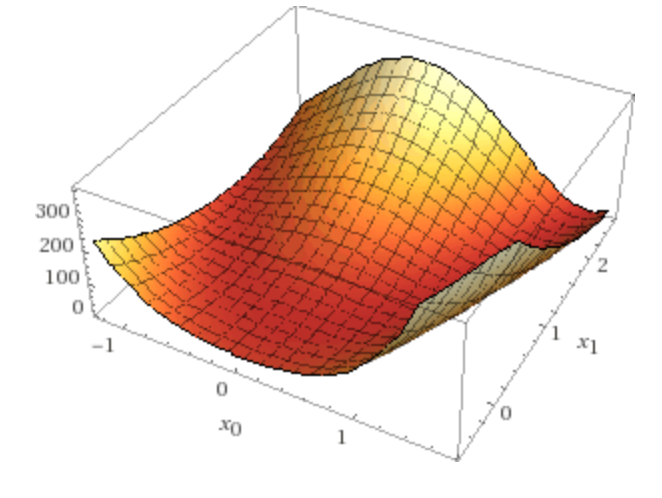
\includegraphics[width=\linewidth]{img/function}
            \captionof{figure}{График функции $f(x)$}
        \end{minipage}
    \end{center}
    
\subsection{Задача 3.1}

\subsubsection{Алгоритм Свенна}
    Прежде, чем переходить к реализации самих алгоритмов поиска экстремума, необходимо найти интервал, где будет находиться стационарная точка. Для этого воспользуемся алгоритмом Свенна:
    
    \begin{enumerate}
        \item Задать произвольно следующие параметры: $x^0$ - начальную точку, $t > 0$ - величину шага. Положить $k = 0$.
        \item Вычислить значение функции в трех точках: $x^0 - t, \quad x^0, \quad x^0 + t$.
        \item Проверить условия окончания:
        \begin{enumerate}
            \item если $f(x^0 - t) \geq f(x^0) \leq f(x^0 + t)$, то начальный интервал неопределенности найден: $[a_0, b_0] = [x^0 - t, x^0 + t]$;
            \item если $f(x^0 - t) \leq f(x^0) \geq f(x^0 + t)$, то функция не является унимодальной, а требуемый интервал неопределенности не может быть найден. Вычисления при этом прекращаются (рекомендуется задать другую начальную точку $x^0$);
            \item если условие окончания не выполняется, то перейти на п. \textbf{4}.
        \end{enumerate}
        \item Определить величину $\bigtriangleup$:
        \begin{enumerate}
            \item если $f(x^0 - t) \geq f(x^0) \geq f(x^0 + t)$, то $\bigtriangleup = t$; $a_0 = x^0$; $x^1 = x^0 + t$; $k=1$;
            \item если $f(x^0 - t) \leq f(x^0) \leq f(x^0 + t)$, то $\bigtriangleup = -t$; $b_0 = x^0$; $x^1 = x^0 - t$; $k=1$;
        \end{enumerate}
        \item Найти следующую точку $x^{k+1} = x^k + 2^k \bigtriangleup$.
        \item Проверить условие убывания функции:
        \begin{enumerate}
            \item если $f(x^{k+1}) < f(x^k)$ и $\bigtriangleup = t$, то $a_0 = x^k$;
            \item если $f(x^{k+1}) < f(x^k)$ и $\bigtriangleup = -t$, то $b_0 = x^k$
            \item если $f(x^{k+1}) \neq f(x^k)$, процедура завершается.
        \end{enumerate}
        в первых двух случаях положить $k = k + 1$ и перейти на п. \textbf{5}
    \end{enumerate}
    При $\bigtriangleup = t$ положить $b_0 = x^{k+1}$, а при $\bigtriangleup = -t$ положить $a_0 = x^{k+1}$. В результате имеем интервал $[a_0, b_0]$ - искомый начальный интервал неопределенности.
    
\subsubsection{Метод деления интервала пополам.}
    Метод относится к последовательным стратегиям и позволяет исключить из дальнейшего рассмотрения на каждой итерации в точности половину текущего интервала неопределенности. Задается начальный интервал неопределенности, а алгоритм уменьшения интервала, являясь, как и в общем случае, «гарантирующим» основан на анализе величин функции в трех точках, равномерно распределенных на текущем интервале. Условия окончания процесса поиска стандартные: поиск заканчивается, когда длина текущего интервала неопределенности оказывается меньше установленной величины. 

\subsubsection{Метод зотолого сечения.}
    Для построения конкретного метода одномерной минимизации, работающего по принципу последовательного сокращения интервала неопределенности, следует задать правило выбора на каждом шаге двух внутренних точек. Конечно, желательно, чтобы одна из них всегда использовалась в качестве внутренней точки и для следующего интервала. Тогда число вычислений функции сократится вдвое и одна итерация потребует расчета только одного нового значения функции. В методе золотого сечения в качестве двух внутренних точек выбирают точки золотого сечения.

    Точка производит \textit{\textbf{«золотое сечение»}} отрезка, если отношение длины всего отрезка к большей части равно отношению большей части к меньшей.

\subsubsection{Метод Фибоначчи.}
    Для построения эффективного метода одномерной минимизации, работающего по принципу последовательного сокращения интервала неопределенности, следует задать правило выбора на каждом шаге двух внутренних точек. Конечно, желательно, чтобы одна из них всегда использовалась в качестве внутренней точки и для следующего интервала. Тогда число вычислений функции сократится вдвое и одна итерация потребует расчета только одного нового значения функции. В методе Фибоначчи реализована стратегия, обеспечивающая максимальное гарантированное сокращение интервала неопределенности при заданном количестве вычислений функции и претендующая на оптимальность. Эта стратегия опирается на числа Фибоначчи.

    \textit{\textbf{Числа Фибоначчи}} определяются по формуле:
    \begin{equation}
        F_0 = F_1, \quad F_k = F_{k-1} + F_{k-2}, \quad k = 2,3,4,...
    \end{equation}
    
    Последовательность чисел Фибоначчи имеет вид: 1, 1, 2, 3, 5, 8, 13, 21, 34, 55, 89, ….
    
\subsection{Задача 3.2}

\subsubsection{Метод квадратичной интерполяции.}

    Метод квадратичной интерполяции (метод Пауэлла) относится к последовательным стратегиям. Задаётся начальная точка и с помощью пробного шага находятся три точки так, чтобы они были как можно ближе к искомой точке минимума. В полученных точках вычисляются значения функции. Затем строится интерполяционный полином второй степени, проходящий через эти три точки. В качестве приближения точки минимума берется точка минимума полинома. Процесс поиска заканчивается, когда полученная точка является наилучшей из трёх опорных точек не более чем на заданную величину.

\subsubsection{Метод кубической интерполяции.}

    Задаётся начальная точка и с помощью серии пробных шагов находятся две точки, первые производные в которых имеют противоположные знаки. По величине функции и её первых производных в полученных точках строится интерполяционный полином третьей степени. В качестве приближения точки минимума берётся точка минимума полинома.  Процесс поиска заканчивается, если производная в точке минимума полинома достаточно мала или процедура становится неэффективной.

\newpage

\section{Практическая реализация}

    Все методы были реализованы на языке программирования \textbf{Kotlin}. Использовался вспомогательный класс \textit{Interval}.
    
    \textbf{Листинг 1.} Класс \textit{Interval}
    \begin{minted}[frame=single, framesep=10pt, fontsize = \footnotesize, linenos=true, breaklines]{kotlin}
data class Interval(var xStart: Float,
                    var xEnd: Float) {

    fun getLength() = (xEnd - xStart).absoluteValue
    
    fun getCenter() = (xEnd + xStart) / 2
    
    override fun toString(): String {
        return "[$xStart, $xEnd]"
    }
}
    \end{minted}
    

\subsection{Задача 3.1}

    \textbf{Листинг 2.} Алгоритм Свенна.
    \begin{minted}[frame=single, framesep=10pt, fontsize = \footnotesize, linenos=true, breaklines]{kotlin}
fun svannMethod(xStart: Float,
                stepSize: Float,
                function: (x: Float) -> Float): Interval {
    PrintUtils.printInfoStart("Svann Method")

    var k = 0
    lateinit var interval: Interval

    val xValues = arrayListOf(xStart)

    val funResultWithoutStepSize = function(xStart - stepSize)
    val funResultOnStart = function(xStart)
    val funResultWithStepSize = function(xStart + stepSize)

    interval = Interval(funResultWithoutStepSize, funResultOnStart)

    if (funResultWithoutStepSize >= funResultOnStart && funResultOnStart <= funResultWithStepSize) {    // step 3.a
        return interval

    } else if (funResultWithoutStepSize <= funResultOnStart && funResultOnStart >= funResultWithStepSize) {     // step 3.b
        throw Exception("Interval can't be found, choose another xStart ($xStart) variable!")

    } else {    // step 4
        var delta = 0.0f
        k += 1

        if (funResultWithoutStepSize >= funResultOnStart && funResultOnStart >= funResultWithStepSize) {  // step 4.a
            delta = stepSize
            interval.xStart = xValues[0]

            xValues.add(k, xStart + stepSize)
        } else if (funResultWithoutStepSize <= funResultOnStart && funResultOnStart <= funResultWithStepSize) { // step 4.b
            delta = -stepSize
            interval.xEnd = xValues[0]

            xValues.add(k, xStart - stepSize)
        }

        while (true) {
            xValues.add(k + 1, (xValues[k] + 2.0.pow(k) * delta).toFloat())     // step 5

            if (function(xValues[k + 1]) >= function(xValues[k])) {
                if (delta > 0) {
                    interval.xEnd = xValues[k + 1]
                } else if (delta < 0) {
                    interval.xStart = xValues[k + 1]
                }
            } else {
                if (delta > 0) {
                    interval.xStart = xValues[k]
                } else if (delta < 0) {
                    interval.xEnd = xValues[k]
                }
            }

            if (function(xValues[k + 1]) >= function(xValues[k])) {
                break
            }
            k += 1
        }
    }

    PrintUtils.printInfoEnd(k, 0, interval)
    return interval
}
    \end{minted}

    \textbf{Листинг 3.} Метод деления интервала пополам.
    \begin{minted}[frame=single, framesep=10pt, fontsize = \footnotesize, linenos=true, breaklines]{kotlin}
fun bisectionMethod(epsilon: Float,
                    interval: Interval,
                    function: (x: Float) -> Float): Float {
    PrintUtils.printInfoStart("Bisection method")

    var k = 0
    var xMiddle = interval.getCenter()

    do {
        val xLeftMiddle = interval.xStart + interval.getLength() / 4
        val xRightMiddle = interval.xEnd - interval.getLength() / 4

        when {
            function(xLeftMiddle) < function(xMiddle) -> {
                interval.xEnd = xMiddle
                xMiddle = xLeftMiddle
            }
            function(xRightMiddle) < function(xMiddle) -> {
                interval.xStart = xMiddle
                xMiddle = xRightMiddle
            }
            else -> {
                interval.xStart = xLeftMiddle
                interval.xEnd = xRightMiddle
            }
        }

        k += 1
    } while (interval.getLength() > epsilon)

    PrintUtils.printInfoEndFunction(k, 0, xMiddle, function)
    return xMiddle
}
    \end{minted}
    
    \textbf{Листинг 4.} Метод золотого сечения.
    \begin{minted}[frame=single, framesep=10pt, fontsize = \footnotesize, linenos=true, breaklines]{kotlin}
fun goldenSectionMethod(epsilon: Float,
                        interval: Interval,
                        function: (x: Float) -> Float): Float {
    PrintUtils.printInfoStart("Golden Section method")

    var k = 0
    val phi = (1 + Math.sqrt(5.0)) / 2

    while (interval.getLength() > epsilon) {
        val z = (interval.xEnd - (interval.xEnd - interval.xStart) / phi).toFloat()
        val y = (interval.xStart + (interval.xEnd - interval.xStart) / phi).toFloat()
        if (function(y) <= function(z)) {
            interval.xStart = z
        } else {
            interval.xEnd = y
        }

        k += 1
    }

    PrintUtils.printInfoEndFunction(k, 0, interval.getCenter(), function)
    return interval.getCenter()
}
    \end{minted}
    
    \textbf{Листинг 5.} Метод Фибоначчи.
    \begin{minted}[frame=single, framesep=10pt, fontsize = \footnotesize, linenos=true, breaklines]{kotlin}
fun fibonacciMethod(eps: Float,
                    interval: Interval,
                    function: (x: Float) -> Float): Float {
    PrintUtils.printInfoStart("Fibonacci method")

    var k = 0

    var y: Float
    var z: Float
    var n = 3
    val fibArr = arrayListOf(1.0, 1.0, 2.0, 3.0)
    var f1 = 2.0
    var f2 = 3.0
    while (fibArr[fibArr.size - 1] < interval.getLength() / eps) {
        fibArr.add(f1 + f2)
        f1 = f2
        f2 = fibArr[fibArr.size - 1]
        ++n
    }
    for (i in 1 until n - 3) {
        y = (interval.xStart + fibArr[n - i - 1] / fibArr[n - i + 1] * (interval.xEnd - interval.xStart)).toFloat()
        z = (interval.xStart + fibArr[n - i] / fibArr[n - i + 1] * (interval.xEnd - interval.xStart)).toFloat()
        if (function(y) <= function(z))
            interval.xEnd = z
        else
            interval.xStart = y

        k += 1
    }

    PrintUtils.printInfoEndFunction(k, timeExecution, interval.getCenter(), function)
    return interval.getCenter()
}
    \end{minted}
    
\subsection{Задача 3.2}

    \textbf{Листинг 6.} Метод квадратичной интерполяции.
    \begin{minted}[frame=single, framesep=10pt, fontsize = \footnotesize, linenos=true, breaklines]{kotlin}
fun quadraticInterpolation(eps: Float,
                           delta: Float,
                           xStart: Float,
                           stepSize: Float,
                           function: (x: Float) -> Float): Float {
    PrintUtils.printInfoStart("Quadratic Interpolation method")

    var a1 = xStart
    var k = 0

    while (true) {
        // Step 2
        var a2 = a1 + stepSize

        // Step 3
        val f1 = function(a1)
        val f2 = function(a2)

        // Step 4
        var a3 = if (f1 > f2) {
            a1 + 2 * stepSize
        } else {
            a1 - 2 * stepSize
        }

        while (true) {
            k += 1

            // Step 5
            val f3 = function(a3)

            // Step 6
            val fMin = min(f1, min(f2, f3))
            val aMin = when (fMin) {
                f1 -> a1
                f2 -> a2
                f3 -> a3
                else -> throw Exception("Cannot find fMin")
            }

            // Step 7
            val det = 2 * ((a2 - a3) * f1 + (a3 - a1) * f2 + (a1 - a2) * f3)
            if (det == 0f) {
                a1 = aMin
            } else {
                val a = ((a2.pow(2) - a3.pow(2)) * f1 + (a3.pow(2) - a1.pow(2)) * f2 + (a1.pow(2) - a2.pow(2)) * f3) / det

                // Step 8
                if (((fMin - function(a)) / function(a)).absoluteValue < eps && ((aMin - a) / a).absoluteValue < delta) { // a)
                    PrintUtils.printInfoEndFunction(k, 0, a1, function)
                    return a
                } else {
                    if (a in a1..a3) { // b)
                        if (a < a2) {
                            a3 = a2
                            a2 = a
                        } else {
                            a1 = a2
                            a2 = a
                        }
                    } else { // c)
                        a1 = a
                        break
                    }
                }
            }
        }
    }
}
    \end{minted}

    \textbf{Листинг 7.} Метод кубической интерполяции.
    \begin{minted}[frame=single, framesep=10pt, fontsize = \footnotesize, linenos=true, breaklines]{kotlin}
fun cubicInterpolation(eps: Float,
                       delta: Float,
                       xStart: Float,
                       stepSize: Float,
                       function: (x: Float) -> Float,
                       derivativeFunction: (x: Float) -> Float): Float {
    PrintUtils.printInfoStart("Cubic Interpolation")

    var a1 = xStart
    var k = 0

    // Step 2
    val df = derivativeFunction(xStart)

    var m = 0f
    var a2 = a1
    // Step 3
    if (df < 0) {
        do {
            a1 = a2
            a2 += m.pow(2) * stepSize
            m += 1f
        } while (derivativeFunction(a1) * derivativeFunction(a2) > 0)
    } else {
        do {
            a1 = a2
            a2 -= m.pow(2) * stepSize
            m += 1f
        } while (derivativeFunction(a1) * derivativeFunction(a2) > 0)
    }

    while (true) {
        k += 1

        // Step 4
        val f1 = function(a1)
        val f2 = function(a2)
        val df1 = derivativeFunction(a1)
        val df2 = derivativeFunction(a2)

        // Step 5
        val z = 3 * (f1 - f2) / (a2 - a1) + df1 + df2
        val w = if (a1 < a2) {
            sqrt(z.pow(2) - df1 * df2)
        } else {
            - sqrt(z.pow(2) - df1 * df2)
        }
        val mu = (df2 + w - z) / (df2 - df1 + 2*w)

        var a = when {
            mu < 0 -> a2
            mu in 0.0..1.0 -> a2 - mu * (a2 - a1)
            mu > 1 -> a1
            else -> throw Exception("Error in range")
        }

        // Step 6
        while (function(a) > function(a1) && ((a - a1) / a).absoluteValue > delta) {
            a -= (a - a1) / 2
        }

        // Step 7
        if (derivativeFunction(a).absoluteValue <= eps && ((a - a1) / a).absoluteValue <= delta) {
            PrintUtils.printInfoEndFunction(k, 0, a, function)
            return a
        } else {
            if (derivativeFunction(a) * derivativeFunction(a1) <= 0) {
                a2 = a1;
                a1 = a;
            } else {
//              a2 = a2;
                a1 = a;
            }
        }

    }
}
    \end{minted}
    
\newpage

\section{Результаты.}
    При последовательном запуске всех алгоритмов со следующими параметрами -
    \begin{equation}
        stepSize = 0.01{\text f}, epsilon = 0.01{\text f}, delta = 0.01{\text f}
    \end{equation}
    были получены следующие результаты:
    
    \textbf{Листинг 8.} Результаты выполнения программ.
    \begin{minted}[frame=single, framesep=10pt, fontsize = \footnotesize, linenos=true, breaklines]{text}
Start Svann Method:
	 Iteration(s): 2
	 Result: [-2.0, 4.0]

Start Bisection method:
	 Iteration(s): 10
	 f(0.12402344) = 2.8125114

Start Golden Section method:
	 Iteration(s): 14
	 f(0.12597115) = 2.8125114

Start Fibonacci method:
	 Iteration(s): 10
	 f(0.13934426) = 2.814969

Start Quadratic Interpolation method:
	 Iteration(s): 3
	 f(0.12498383) = 2.8125

Start Cubic Interpolation:
	 Iteration(s): 2
	 f(0.125) = 2.8125
	 \end{minted}
 
Все результаты с небольшой погрешностью совпадают с результатами полученными с помощью сервиса WolframAlpha.com в пункте 3. Наилучшая точность получена с помощью метода кубической инерполяции.

\end{document} 